% Arsitektur final pipeline ekstraksi field KYC.
% Kompilasi: pdflatex architecture.tex
\documentclass[border=12pt,tikz]{standalone}
\usepackage[T1]{fontenc}
\usepackage{amsmath}
\usepackage{tikz}
\usetikzlibrary{arrows.meta,positioning,fit,backgrounds,calc}

\definecolor{cInput} {HTML}{E8EAED}
\definecolor{cOcr}   {HTML}{CFE2F3}
\definecolor{cModel} {HTML}{D9EAD3}
\definecolor{cRule}  {HTML}{FCE5CD}
\definecolor{cOut}   {HTML}{F4CCCC}
\definecolor{cLine}  {HTML}{5F6368}
\definecolor{cMuted} {HTML}{80868B}

\begin{document}
\sffamily
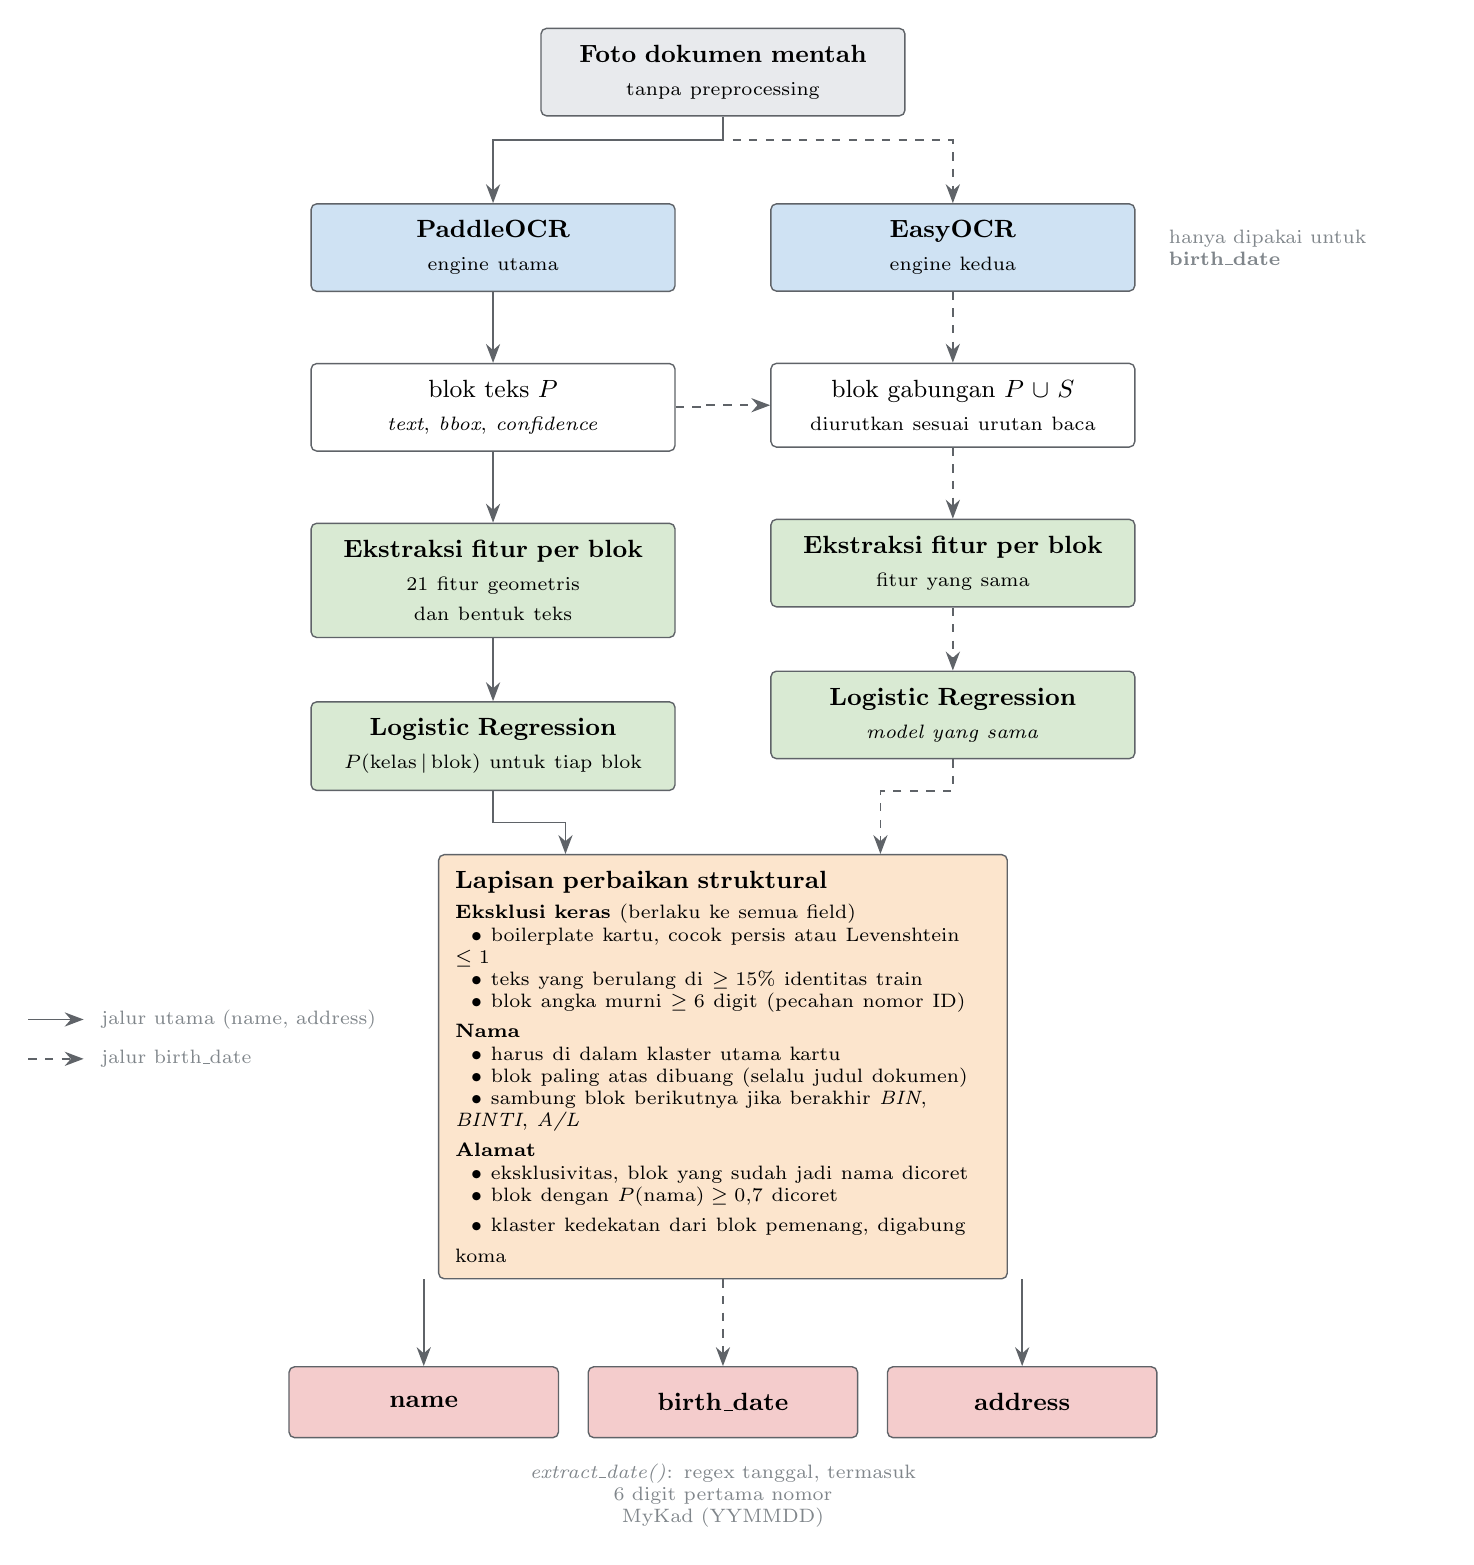
\begin{tikzpicture}[
  font=\small,
  node distance=8mm,
  box/.style={
    rounded corners=2pt, draw=cLine, line width=0.5pt,
    align=center, inner sep=6pt, minimum height=9mm, text width=42mm},
  input/.style ={box, fill=cInput},
  ocr/.style   ={box, fill=cOcr},
  model/.style ={box, fill=cModel},
  rule/.style  ={box, fill=cRule, text width=68mm, align=left},
  outbox/.style={box, fill=cOut, text width=30mm},
  ar/.style    ={-{Stealth[length=2.4mm]}, draw=cLine, line width=0.6pt},
  ard/.style   ={ar, dashed},
  note/.style  ={align=left, text=cMuted, font=\scriptsize, text width=46mm},
]

% ---------------------------------------------------------------- input
\node[input] (img) {\textbf{Foto dokumen mentah}\\[1pt]{\scriptsize tanpa preprocessing}};

% ---------------------------------------------------------------- OCR
\node[ocr, below left=11mm and 6mm of img.south]  (pad) {\textbf{PaddleOCR}\\[1pt]{\scriptsize engine utama}};
\node[ocr, below right=11mm and 6mm of img.south] (easy){\textbf{EasyOCR}\\[1pt]{\scriptsize engine kedua}};

\node[note, right=3mm of easy.east, text width=34mm]
  {hanya dipakai untuk \textbf{birth\_date}};

% blocks
\node[box, fill=white, below=9mm of pad, text width=42mm] (bp)
  {blok teks $P$\\[1pt]{\scriptsize \textit{text}, \textit{bbox}, \textit{confidence}}};
\node[box, fill=white, below=9mm of easy, text width=42mm] (bs)
  {blok gabungan $P \cup S$\\[1pt]{\scriptsize diurutkan sesuai urutan baca}};

% ---------------------------------------------------------------- features + model
\node[model, below=9mm of bp]  (f1) {\textbf{Ekstraksi fitur per blok}\\[1pt]{\scriptsize 21 fitur geometris dan bentuk teks}};
\node[model, below=9mm of bs]  (f2) {\textbf{Ekstraksi fitur per blok}\\[1pt]{\scriptsize fitur yang sama}};

\node[model, below=8mm of f1] (m1) {\textbf{Logistic Regression}\\[1pt]{\scriptsize $P(\textrm{kelas}\,|\,\textrm{blok})$ untuk tiap blok}};
\node[model, below=8mm of f2] (m2) {\textbf{Logistic Regression}\\[1pt]{\scriptsize \textit{model yang sama}}};

% ---------------------------------------------------------------- structural layer
\node[rule, below=10mm of $(m1.south)!0.5!(m2.south)$, anchor=north] (struct) {
  \textbf{Lapisan perbaikan struktural} \\[3pt]
  {\scriptsize
  \textbf{Eksklusi keras} (berlaku ke semua field)\\
  \hspace*{2mm}$\bullet$ boilerplate kartu, cocok persis atau Levenshtein $\le 1$\\
  \hspace*{2mm}$\bullet$ teks yang berulang di $\ge 15\%$ identitas train\\
  \hspace*{2mm}$\bullet$ blok angka murni $\ge 6$ digit (pecahan nomor ID)\\[3pt]
  \textbf{Nama}\\
  \hspace*{2mm}$\bullet$ harus di dalam klaster utama kartu\\
  \hspace*{2mm}$\bullet$ blok paling atas dibuang (selalu judul dokumen)\\
  \hspace*{2mm}$\bullet$ sambung blok berikutnya jika berakhir \textit{BIN}, \textit{BINTI}, \textit{A/L}\\[3pt]
  \textbf{Alamat}\\
  \hspace*{2mm}$\bullet$ eksklusivitas, blok yang sudah jadi nama dicoret\\
  \hspace*{2mm}$\bullet$ blok dengan $P(\text{nama}) \ge 0{,}7$ dicoret\\
  \hspace*{2mm}$\bullet$ klaster kedekatan dari blok pemenang, digabung koma
  }};

% ---------------------------------------------------------------- outputs
\node[outbox, below=11mm of struct.south, xshift=-38mm] (oname) {\textbf{name}};
\node[outbox, below=11mm of struct.south, xshift=0mm]   (odate) {\textbf{birth\_date}};
\node[outbox, below=11mm of struct.south, xshift=38mm]  (oaddr) {\textbf{address}};

\node[note, below=2mm of odate, text width=52mm, align=center]
  {\textit{extract\_date()}: regex tanggal, termasuk\\ 6 digit pertama nomor MyKad (YYMMDD)};

% ---------------------------------------------------------------- arrows
\draw[ar]  (img.south) -- ++(0,-3mm) -| (pad.north);
\draw[ard] (img.south) -- ++(0,-3mm) -| (easy.north);
\draw[ar]  (pad)  -- (bp);
\draw[ard] (easy) -- (bs);
\draw[ar]  (bp)   -- (f1);
\draw[ard] (bs)   -- (f2);
\draw[ar]  (f1)   -- (m1);
\draw[ard] (f2)   -- (m2);
\draw[ar]  (m1.south) -- ++(0,-4mm) -| ([xshift=-20mm]struct.north);
\draw[ard] (m2.south) -- ++(0,-4mm) -| ([xshift=20mm]struct.north);

\draw[ar]  ([xshift=-38mm]struct.south) -- (oname.north);
\draw[ard] (struct.south)               -- (odate.north);
\draw[ar]  ([xshift=38mm]struct.south)  -- (oaddr.north);

% also feed the primary blocks into the merged path
\draw[ard] (bp.east) -- ++(4mm,0) |- (bs.west);

% ---------------------------------------------------------------- legend
\begin{scope}[shift={($(struct.west)+(-52mm,6mm)$)}]
  \draw[ar]  (0,0) -- (7mm,0);
  \node[right=1mm of {(7mm,0)}, font=\scriptsize, text=cMuted, anchor=west]
    {jalur utama (name, address)};
  \draw[ard] (0,-5mm) -- (7mm,-5mm);
  \node[right=1mm of {(7mm,-5mm)}, font=\scriptsize, text=cMuted, anchor=west]
    {jalur birth\_date};
\end{scope}

\end{tikzpicture}
\end{document}
